\section{Аналитический раздел}
\subsubsection{Описание предметной области}
FTP — протокол передачи файлов по сети, является одним из старейших прикладных протоколов, появившихся задолго до HTTP, и даже до TCP/IP, в 1971 году; в первое время он работал поверх протокола NCP. 
Он и сегодня широко используется для распространения ПО и доступа к удалённым хостам. 
В отличие от TFTP, гарантирует передачу (либо выдачу ошибки) за счет применения квотируемого протокола.

Протокол построен на архитектуре «клиент-сервер» и использует разные сетевые соединения для передачи команд и данных между клиентом и сервером. 
Пользователи FTP могут пройти аутентификацию, передавая логин и пароль открытым текстом, или же, если это разрешено на сервере, они могут подключиться анонимно. 
Можно использовать протокол SSH для безопасной передачи, скрывающей (шифрующей) логин и пароль, а также шифрующей содержимое.

Первые клиентские FTP-приложения были интерактивными инструментами командной строки, реализующими стандартные команды и синтаксис. 
С тех пор были разработаны графические пользовательские интерфейсы для многих используемых по сей день операционных систем. 
Среди этих интерфейсов как компоненты программы общего веб-дизайна вроде Microsoft Expression Web, так и специализированные FTP-клиенты (например, FileZilla).

\subsubsection{Архитектура системы}
Клиент - программа для упрощения доступа к FTP серверу. 
В зависимости от назначения может либо предоставлять пользователю простой доступ к удаленному FTP-серверу в режиме текстовой консоли, беря на себя только работу по пересылке команд пользователя и файлов, либо отображать файлы на удаленном сервере как если бы они являлись частью файловой системы компьютера пользователя, либо и то и другое. 
В последних двух случаях FTP-клиент берет на себя задачу интерпретации действий пользователя в команды протокола FTP, тем самым давая возможность использовать протокол передачи файлов без ознакомления со всеми его премудростями. 
В простейшем для пользователя (но при этом наиболее комплексном) случае FTP-клиент представляет из себя эмулятор файловой системы, которая просто находится на другом компьютере. 
С этой файловой системой можно совершать все привычные пользователю действия: копировать файлы с и на сервер, удалять файлы, создавать новые файлы. 
В отдельных случаях возможно также открытие файлов - для просмотра, запуска программ, редактирования. Необходимо учитывать лишь, что открытие файла подразумевает его предварительное скачивание на компьютер пользователя Благодаря распространенности протокола FTP, простые (с точки зрения реализации) FTP-клиенты есть практически в каждой операционной системе. 
Однако использование этих клиентов требует навыков использования консоли, а также знания команд протокола для общения с сервером. 
Так в Windows такой утилитой является ftp.exe. 
Во многих сборках Linux так же есть утилита ftp. 
Файловая система на удаленном сервере как правило имеет настройки прав доступа для различных пользователей. 
Так, например, анонимным пользователям могут быть доступны лишь некоторые файлы, о существовании других пользователи знать не будут. 
Другой группе пользователей могут быть доступны другие файлы или, например, в дополнение к правам на чтение файлов, могут быть также даны права на запись новых или обновление имеющихся файлов. 
Диапазон вариантов прав доступа зависит от операционной системы и программного обеспечения каждого конкретного FTP-сервера. 
Как правило, разделяют права на просмотр содержимого папки (т.е. возможность получить список содержащихся в ней файлов), на чтение файла(ов), на запись (создание, удаление, обновление) файла(ов). 
Для авторизации FTP-сервер, при подключении к нему FTP-клиента, запрашивает у последнего имя пользователя и пароль. 
Большинство FTP-клиентов в свою очередь запрашивают эти данные у пользователя в интерактивном режиме. 
Есть так же и другой способ указать эти данные, включив их в URL FTP-сервера. 
Так, например, в строке://setevoy:pass@ftp.someserver.com:// - указание того, что мы используем протокол FTP, где:
\begin{enumerate}
	\item setevov - имя пользователя;
	\item : - разделитель;
	\item pass - пароль;
	\item @ - разделитель аутентификационной информации и адреса сервера;
	\item someserver.ru - адрес FTP - сервера;
\end{enumerate}

Нередки случаи, когда такой метод указания имени пользователя и пароля является единственным, который поддерживает FTP-клиент.

\subsection{Протокол прикладного уровня}
Протокол пересылки файлов ftp - это протокол прикладного уровня стека TCP/IP . 
Работа этого протокола основана на архитектуре “клиент-сервер”. 
Команды и данные, в отличие от большинства других протоколов передаются по разным портам. 
Порт 20 используется для передачи данных, порт 21 для передачи команд. Основные команды:. 
Как правило, эта команда открывает сессию FTP между клиентом и сервером. 
Аргументом команды является имя (идентификатор) пользователя для работы с файловой системой. 
Эта команда может подаваться не только в начале, но и в середине сессии, если, например, пользователь желает изменить идентификатор, от имени которого будут проводиться действия. 
При этом все переменные, относящиеся к старому идентификатору, освобождаются. 
Если во время изменения идентификатора происходит обмен данными, обмен завершается со старым идентификатором пользователя. 
Данная команда подается после ввода идентификатора пользователя и, в качестве аргумента содержит пароль пользователя. 
Напомним, что данные аутентификации FTP передаются по сети открытым текстом, поэтому для обеспечения защищенности канала пользователю необходимо предпринимать дополнительные меры. 
Команда позволяет пользователям работать с различными каталогами удаленной файловой системы. 
Аргументом команды является строка, указывающая путь каталога удаленной файловой системы, в котором желает работать пользователь. 
Команда реинициализации. Эта команда очищает все переменные текущего пользователя, сбрасывает параметры соединения. 
Если в момент подачи команды происходит передача данных, передача продолжается и завершается с прежними параметрами. 
Команда закрывает управляющий канал. 
Если в момент подачи команды происходит передача данных, канал закрывается после окончания передачи данных. 
Команды управления потоком устанавливают параметры передачи данных. 
Все параметры, описываемые этими командами имеют значение по умолчанию, поэтому команды управления потоком используются только тогда, когда необходимо изменить значение параметров передачи, используемых по умолчанию. 
Команды управления потоком могут подаваться в любом порядке, но все они должны предшествовать командам FTP-сервиса. 
Из команд управления потоком данных следует выделить следующие:. Команда назначает адрес и порт хоста, который будет использоваться как активный участник соединения по каналу передачи данных. Аргументами команды являются 32-битный IP адрес и 16-битный номер порта соединения. 
Эти значения разбиты на шесть 8-битных полей и представлены в десятичном виде: h1, h2, h3, h4, p1, p2, где hN - байты адреса (от старшего к младшему), а pN - байты порта (от старшего к младшему). 
Эта команда отправляется модулю, который будет играть пассивную роль, в передаче данных («слушать» соединение). Ответом на данную команду должна быть строка, содержащая адрес и порт хоста, находящиеся в режиме ожидания соединения в формате команды PORT - «h1, h2, h3, h4, p1, p2». 
Команды TYPE, STRU, MODE определяют, соответственно, тип передаваемых данных (ASCII, Image и другие), структуру или формат передачи данных (File, Record, Page), способ передачи (Stream, Block и другие). 
Использование этих команд очень важно при построении взаимодействия в гетерогенных средах и весьма отличающихся операционных и файловых систем взаимодействующих хостов. 
Команды FTP-сервиса определяют действия, которые необходимо произвести с указанными файлами. 
Как правило, аргументом команд этой группы является путь к файлу. Синтаксис указанного пути должен удовлетворять требованиям формата файловой системы обработчика команды. 
Из команд FTP-сервиса можно выделить следующие: 
Эта команда указывает модулю «Программа передачи данных сервера» передать копию файла, заданного параметром этой команды, модулю передачи данных на другом конце соединения. 
Команда указывает модулю «Программа передачи данных сервера» принять данные по каналу передачи данных и сохранить их как файл, имя которого задано параметром этой команды. 
Если такой файл уже существует, он будет замещен новым, если нет, будет создан новый. Команды RNFR и RNTO должны следовать одна за другой. 
Первая команда содержит в качестве аргумента старое имя файла, вторая - новое. Последовательное применение этих команд переименовывает файл.
Команда предписывает серверу прервать выполнение предшествующей сервисной команды (например, передачу файла) и закрыть канал передачи данных. 
Команда DELE удаляет указанный файл. Команды MKD и RMD, соответственно, создают и удаляют указанный в аргументе каталог. 
При помощи команд LIST и NLST можно получить список файлов в указанном каталоге.

\subsection{Протокол транспортного уровня}
Транспортный уровень (англ. Transport layer) - 4-й уровень сетевой модели OSI предназначен для доставки данных без ошибок, потерь и дублирования в той последовательности, как они были переданы. 
При этом не важно, какие данные передаются, откуда и куда, то есть он предоставляет сам механизм передачи. 
Transmission Control Protocol (TCP) (протокол управления передачей) - один из основных сетевых протоколов Интернета, предназначенный для управления передачей данных в сетях и подсетях TCP/IP. TCP - это транспортный механизм, предоставляющий поток данных, с предварительной установкой соединения, за счёт этого дающий уверенность в достоверности получаемых данных, осуществляет повторный запрос данных в случае потери данных и устраняет дублирование при получении двух копий одного пакета (см. также T/TCP). 
В отличие от UDP гарантирует, что приложение получит данные точно в такой же последовательности, в какой они были отправлены, и без потерь. 
Реализация TCP, как правило, встроена в ядро системы, хотя есть и реализации TCP в контексте приложения.

\subsection{Активный и пассивный режим}
В активном режиме FTP клиент соединяется с произвольного непривилегированного порта (N > 1024) к FTP серверному командному порту 21. 
Затем, клиент начинает слушать порт N+1 и посылать FTP команду PORT N+1 на FTP сервер. 
В ответ, сервер соединяется с указанным портом данных клиента из своего локального порта данных 20. (рисунок \ref{fig:1})
% TODO: \usepackage{graphicx} required
\begin{figure}[H]
	\centering
	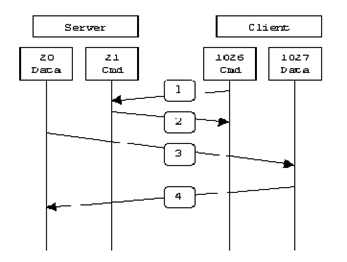
\includegraphics[width=0.7\linewidth]{src/img/1}
	\caption{Принцип работы ftp}
	\label{fig:1}
\end{figure}

В пассивном режиме FTP клиент инициирует оба соединения с сервером, решая проблему с фаерволами, которые фильтруют входящий порт данных клиента. 
При открытии FTP соединения, клиент локально открывает два непривилегированных порта (N > 1024 и N+1). 
Первый порт контактирует с сервером на порт 21, но вместо того, чтобы затем выдать команду PORT и позволить серверу в ответ соединиться с его портом данных, клиент выдает команду PASV. 
В результате сервер открывает произвольный непривилегированный порт (P > 1024) и посылает клиенту команду PORT P. 
Затем, для передачи данных, клиент инициирует соединение от порта N+1 к порту P на сервере.
